% !TEX TS-program = pdflatex
% !TEX encoding = UTF-8 Unicode

% Author: Michael Wagener

\documentclass[11pt]{article} % use larger type; default would be 10pt

\usepackage{pgf}
\usepackage{tikz}
\usetikzlibrary{arrows,automata,shapes}
\usetikzlibrary{decorations.pathmorphing} % LATEX and plain TEX when using Tik Z

\usepackage[utf8]{inputenc} % set input encoding (not needed with XeLaTeX)
\usepackage{geometry} % to change the page dimensions
\geometry{a4paper} % or letterpaper (US) or a5paper or....
\geometry{margin=15mm} % for example, change the margins to 2 inches all round
%\usepackage[ngerman]{babel}

\usepackage{booktabs} % for much better looking tables
\usepackage{array} % for better arrays (eg matrices) in maths
\usepackage{paralist} % very flexible & customisable lists (eg. enumerate/itemize, etc.)
\usepackage{verbatim} % adds environment for commenting out blocks of text & for better verbatim
\usepackage{subfig} % make it possible to include more than one captioned figure/table in a single float
\usepackage{listings}
\usepackage[obeyspaces,spaces]{url} % https://tex.stackexchange.com/questions/164446/how-to-typeset-a-file-path

\usepackage{float}  % https://en.wikibooks.org/wiki/LaTeX/Floats,_Figures_and_Captions
%\floatstyle{boxed} 
\restylefloat{figure}
\usepackage{wrapfig}

\usepackage{scrextend} % für addmargin
\usepackage{color}
\definecolor{mark}{rgb}{0.8,0.2,0.2} % 1=weiß, 0=schwarz
\definecolor{rowcolor}{rgb}{0.94, 0.97, 1.0}

\author{Michael Wagener, JCNS-1}
\title{SAS Scatter2 \\[1ex] {\large User documentation}}

\usepackage{fancyhdr} % This should be set AFTER setting up the page geometry
\pagestyle{fancy} % options: empty , plain , fancy
\renewcommand{\headrulewidth}{0pt} % customise the layout...
\lhead{}\chead{\textbf{SAS Scatter2 Calculations}}\rhead{\today}
\lfoot{Michael Wagener}\cfoot{\thepage}\rfoot{JCNS-1}

\usepackage{sectsty}
\allsectionsfont{\sffamily\mdseries\upshape} % (See the fntguide.pdf for font help)
% (This matches ConTeXt defaults)

%%% ToC (table of contents) APPEARANCE
\usepackage[nottoc,notlof,notlot]{tocbibind} % Put the bibliography in the ToC
\usepackage[titles,subfigure]{tocloft} % Alter the style of the Table of Contents
\renewcommand{\cftsecfont}{\rmfamily\mdseries\upshape}
\renewcommand{\cftsecpagefont}{\rmfamily\mdseries\upshape} % No bold!

\usepackage{longtable} % Tabellen über mehrere Seiten
\usepackage{multirow} % multirow/multicolumn
\usepackage{colortbl} % farbige Tabellenzellen
%\setlength{\LTpre}{0pt} % Remove whitespace befor and after longtables
%\setlength{\LTpost}{0pt}

\usepackage{tabularx}
\newcolumntype{L}[1]{>{\raggedright\arraybackslash}p{#1}} % linksbündig mit Breitenangabe
\newcolumntype{C}[1]{>{\centering\arraybackslash}p{#1}} % zentriert mit Breitenangabe
\newcolumntype{R}[1]{>{\raggedleft\arraybackslash}p{#1}} % rechtsbündig mit Breitenangabe
\newcommand{\ltab}{\raggedright\arraybackslash} % Tabellenabschnitt linksbündig
\newcommand{\ctab}{\centering\arraybackslash} % Tabellenabschnitt zentriert
\newcommand{\rtab}{\raggedleft\arraybackslash} % Tabellenabschnitt rechtsbündig
% https://de.wikibooks.org/wiki/LaTeX-W%C3%B6rterbuch:_tabular


\setlength{\tabcolsep}{1mm} % Setzt den Längenwert von {Abstand zwischen den Spalten einer Tabelle} auf den Wert 1mm
\setcounter{tocdepth}{2} % Tiefe des Inhaltsverzeichnisses

\begin{document}

\maketitle
\tableofcontents % toc anzeigen

\begin{figure}[b] % die History Tabelle am unteren Seitenrand der ersten Seite anzeigen...
\begin{longtable}{|p{2.7cm}|p{2.6cm}|p{10.3cm}|}
\caption{Document revision history} \\
\hline\rowcolor{rowcolor}{\bf Date} & {\bf Author} & {\bf Short description} \\
\endfirsthead
\hline
03. Dec 2021 & M.Wagener & Start with a copy of a former version. \\ \hline
18. Jan 2022 & M.Wagener & Continue writing and insert screenshots. \\ \hline
04. Feb 2022 & M.Wagener & Finish chapter 2 and start with chapter 3. \\ \hline
04. Mar 2022 & M.Wagener & Add directory infos of the git and work on the AI part. \\ \hline
08. Dec 2022 & M.Wagener & Upload to github. \\ \hline
\end{longtable}

\centerline{All sources saved at https://iffgit.fz-juelich.de/wagener/sas-crystal (only private access)}
%\centerline{If you want to have access, please contact m.wagener@fz-juelich.de}
\centerline{Snapshots on https://github.com/MichaelWagener/CrystalScatter with global access}
\end{figure}

\clearpage % neue Seite beginnen


\section{Preface}

The request was to convert a Pascal program for crystal calculations\footnote{Executable download not working anymore, please contact s.foerster@fz-juelich.de}
%from http://www.bzkg.uni-bayreuth.de/de/download/index.html}
to a usable C++ routine and run on a GPU.

During the development the GUI and the internals were changed more than once. But now the system becomes better and seems to be useful, so I marked it with the number {\it 2} in the name. This documentation address the users, another documentation will be written for developers to explain the internals.

The software is written with the Qt library, so that it can run under windows and linux without changes in the source. {\it Due to the used compiler, a GPU cannot be used under Windows. But this is under development.} All screenshots are made on a windows system. It is possible that some parts of the screenshots differs from the current look of the program, it will be developed and the screenshots are not updated every time.

\subsection{Installation and usage hints}

The program can be used under different systems:
\begin{itemize}\itemsep0pt
\item {\bf Windows} (Standalone) \\
	the program can be compiled as one executable file for Windows (10 or later, 64bit). This can be used on your local system without any other software installed.
\item {\bf Windows} (from source) \\
	{\bf Linux} (from source) \\
	{\bf MacOS} (from source) \\
	you can get access to the git system, where the source is available. Then you have to install the Qt development environment and some other libraries\footnote{{\bf FFTW3} for FFTs, if installed this replaces a simple internal code. {\bf HDF5} to read this datatype} if you need the functionality. Then you can compile this program and use it.
\item {\bf Android} (Tablet) \\
	it is possible to compile the program for this system.
\item {\bf IOS} (Tablet) \\
	at the moment I'm not able to compile for this system.
\end{itemize}

\clearpage
\section{GUI}

\centerline{\bf Partly older screenshots in this document}
\centerline{ }

After the start of the program you get this screen, the red and green lines are only for this documentation:

\begin{figure}[H]
 \centering
 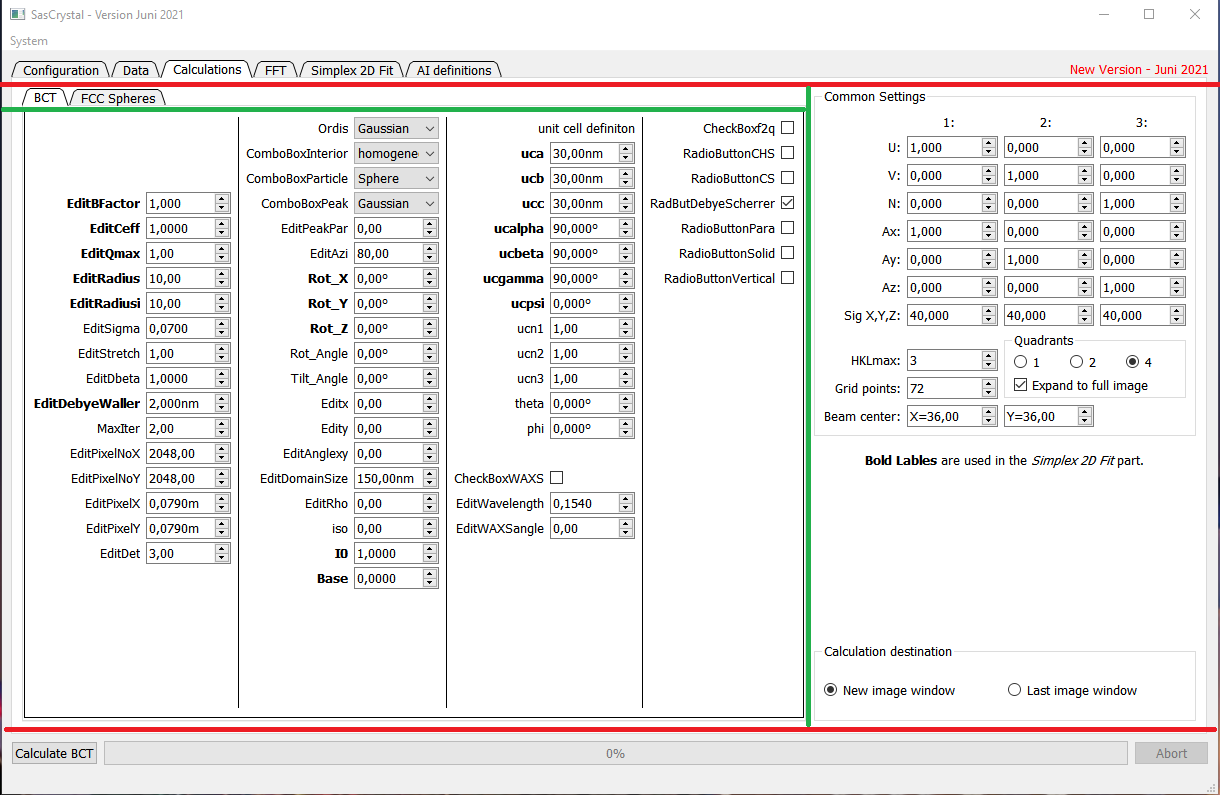
\includegraphics[width=0.96\textwidth]{main-calc-start-lines.png}
 \caption{Calculation parameter overview after startup.}
 \label{fig:calcstart}
\end{figure}


\subsection{Calculation tab}

As you see in Figure \ref{fig:calcstart} the main screen consists of three parts (divided by the red lines, from top to bottom):
\begin{itemize}\itemsep0pt
\item the menu bar and the upper tab selection
\item the area with many values
\item the calculation button with the progress bar at the bottom
\end{itemize}
Each of these parts will be described in this chapter.

\subsubsection{Menubar and selection tabs}

There is only one menu defined in this program.

\begin{wrapfigure}{r}{0.31\textwidth}
  \begin{center}
    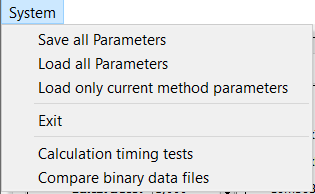
\includegraphics[width=0.30\textwidth]{main-menu.png}
  \end{center}
 \caption{Main menu.}
 \label{fig:mainmenu}
\end{wrapfigure}
There you can save and load the parameters for the calculations. These are stored in a text file in a Windows INI Format. Each file contains all values for all methods together with the settings of the AI tab. With the third menu entry ({\it Load only current method parameters}) only the parameters from the current visible calculation method are loaded. In this case the global parameters (inputs on the right side of the main screen) are not loaded.

The menu entry {\it Calculation timing tests} can be used to document the calculation speed of the current computer. More is described later.

The last menu entry {\it Compare binary data files} can be used to compare data files saved from this program with different calculations or different computers.

Just below the menu bar you can select the different information pages of the program. These are described in the next sections.

\subsubsection{Calculation button and progress bar}

At the bottom left of the program GUI is the button to start the calculation of the current simulation image. The progress bar shows the calculation progress. If the calculation is performed on the CPU, it can be aborted with the button on the right. The update of the progress bar and the checking of the abort button will be done every second. If you click the abort button, the calculation threads will be terminated but it can take some seconds until the threads will stop and the image window is shown\footnote{Sometimes it is possible that the program crashed at this point. I didn't know why but I'll work on it.}. The same procedure is used to stop the calculation after a specified time limit (see Configuration tab).

If the calculation is performed on the GPU, the abort button will be disabled because this function is not available.

\subsubsection{Common settings at the right side of the GUI}

This is the right side of the vertical green line. In the upper part the values for the vectors can be modified and below are some other inputs:
\begin{itemize}\itemsep0pt
\item $\vec{U}, \vec{V}$, $\vec{N}$: Crystal orientation
\item $\vec{Ax}, \vec{Ay}, \vec{Az}$: Peak shape directions
\item $sig_{x}, sig_{y}, sig_{z}$: 4 / Domain size
\item HKLmax: defines the number of calculation iterations and has a significant effect on the calculation time.
\item Grid points: number of pixel of one quadrant of the generated image. The 72 in the screenshot results in an image of 144*144 pixel.
\item Beam center: the x and y pixel position in the grid (one quarter of the result image) of the beam center. These values are used during calculation to move the circular center out of the image center.
\item Quadrants: here you can select, if only one quadrant(1) or the half(2) of the image or the full image(4) are calculated. If the checkbox {\it Expand to full image} is checked, the rest of the image is mirrored over the center to generate allways a full image. This is only usefull if the beam center ist set to zero.
\end{itemize}

On the lower part you can select if the calculated image will be shown in a new window or to overwrite the last image window.

Between these inputs the filename of the loaded parameters will be displayed after loaded.

\subsubsection{Method parameters in the left part of the GUI}

This is the left side of the vertical green line. This part contains two informations: the current calculation method can be selected at the top of this area (above the horizontal green line). The rest contains all values used for this calculation. The number of digits and the minimal and maximal values possible can be set (1) inside the source code of the program and (2) from a special configuration file, described in the Appendix of this document.

All values with a bold label can be used in the Simplex 2D Fit algorithm.

\clearpage
\subsection{Configuration tab}

In the configuration tab there are many groups of settings described here.
\begin{figure}[H]
 \centering
 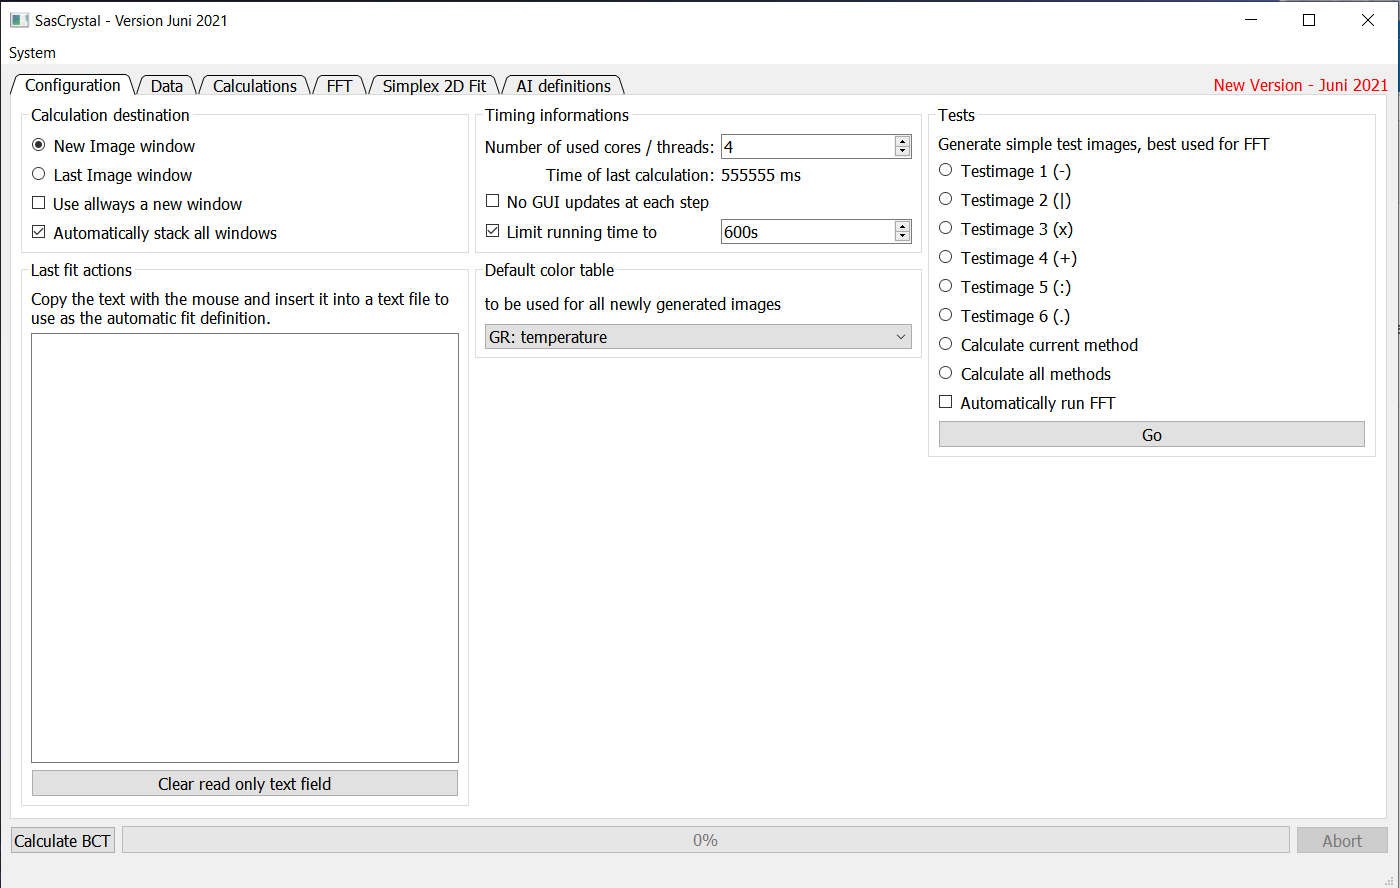
\includegraphics[width=0.96\textwidth]{main-config-start.png}
 \caption{Configuration view after startup.}
 \label{fig:configstart}
\end{figure}
\begin{itemize}\itemsep0pt
\item Calculation destination \\
	Here you can select the destination of the next calculated image (a new window or the last used one). \\
	If the checkbox {\it Automatically stack all windows} is checked, then each new image window is placed at the right side of the last one. If the screen is filled horizontally, the next row will be started below the images. If the screen is vertically filled, the program restarts at the top. But then you might have trouble to find the correct image (see next: Data tab). \\
	If the checkbox {\it Use allways a new checkbox} is checked, then the above selected destination is ignored and each calculated image is placed in a new image window.
\item Last fit actions \\
	In this text field the program writes all actions performed in the Simplex 2D Fit tab. This is useful, if you want to perform an automatic fit to get the correct syntax and to replay what you've done before. With the button under the text field you can clear this readonly field.
\item Timing informations \\
	Here the used number of threads (or GPU) can be set. {\bf Imoprtant note:} if a parameter set is loaded, the number of used threads is taken from the parameter file. So change this only after parameter loading. \\
	The time of the last calculation is shown at the status bar for a few seconds but shown here until the next calculation overwrites it. \\
	Disabling the GUI updates might speed up the calculation time if working over the network (via ssh and vpn). \\
	The calculation time limit (if enabled) can be set to a number of seconds. After this time the calculation thread is stopped and the image displayed contains the values up to this time, the rest of the data is zero. This is the same procedure used by the Abort button (see above).
\item Default color table \\
	All image windows will start with this color table. Inside each of the image windows you can change the color table independently.
\item Tests \\
	Here you can generate some special test images to check the FFT calculations. It was implemented during the FFT programming but now it's seldom used.
\end{itemize}


\subsection{Data tab}

\begin{figure}[H]
 \centering
 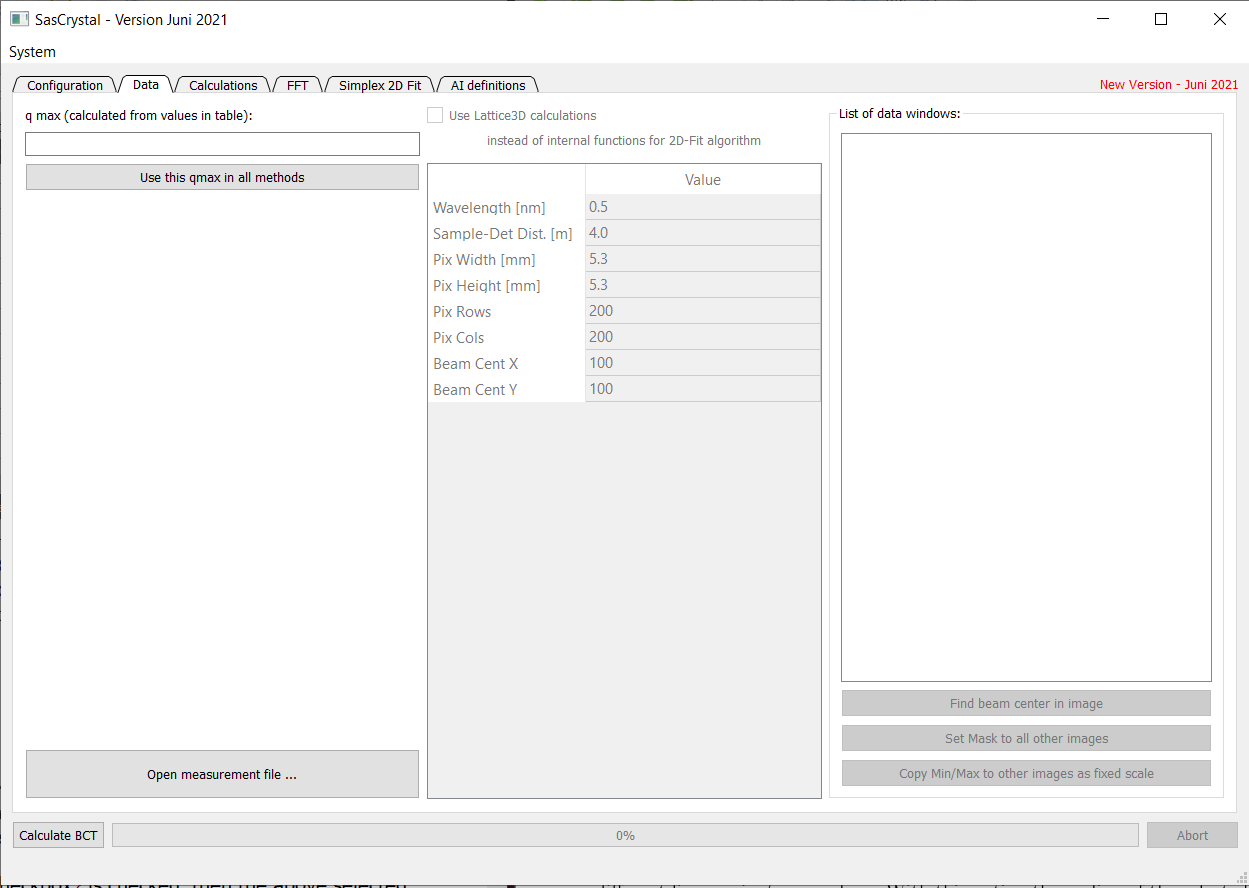
\includegraphics[width=0.96\textwidth]{main-data-start.png}
 \caption{Data view after startup.}
 \label{fig:datastart}
\end{figure}
Some parts of this are historical and may be changed in future.

The essetial button in the lower left part of this tab ({\it open measueremtn file ...}) is used to open files from real measurements for the fit algorithm. You can select different data types (file extensions), the data is loaded and displayed in a new image window. If available some informations from the data file header are displayed in the middle of this tab. All known header informations are stored in the meta informations of the image window.

In the right list all image windows are listed and a klick on an entry rises the image window on top of all other windows. So you can find them. {\it The buttons below this list are only enabled if a KWS image is selected}:
\begin{itemize}\itemsep0pt
\item Find beam center in image \\
	All KWS images have {\it zero pixels} at the corners and at the beam center. The pixel in the middle are searched and the middle point of this region is the beam center. This point can be used for further calculations.
\item Set Mask to all other images (only enabled if more than one image window is open) \\
	This will generate a new image for each of the images in the list not selected. The image will be taken from the original image but all pixel the KWS image has zeros, set to zero.
\item Copy Min/Max to other images as fixed scale (only enabled if more than one image window is open) \\
	Most times the image scaling will be logarithmic. So it is not so easy to compare images visually if they have different linear min / max values. With this option the scaling of the selected image is copied to all other images as a fixed scaling so that all images have the same visual scaling.
%\item Save all windows ...
\end{itemize}


\subsection{FFT tab}

\begin{figure}[h]
 \centering
 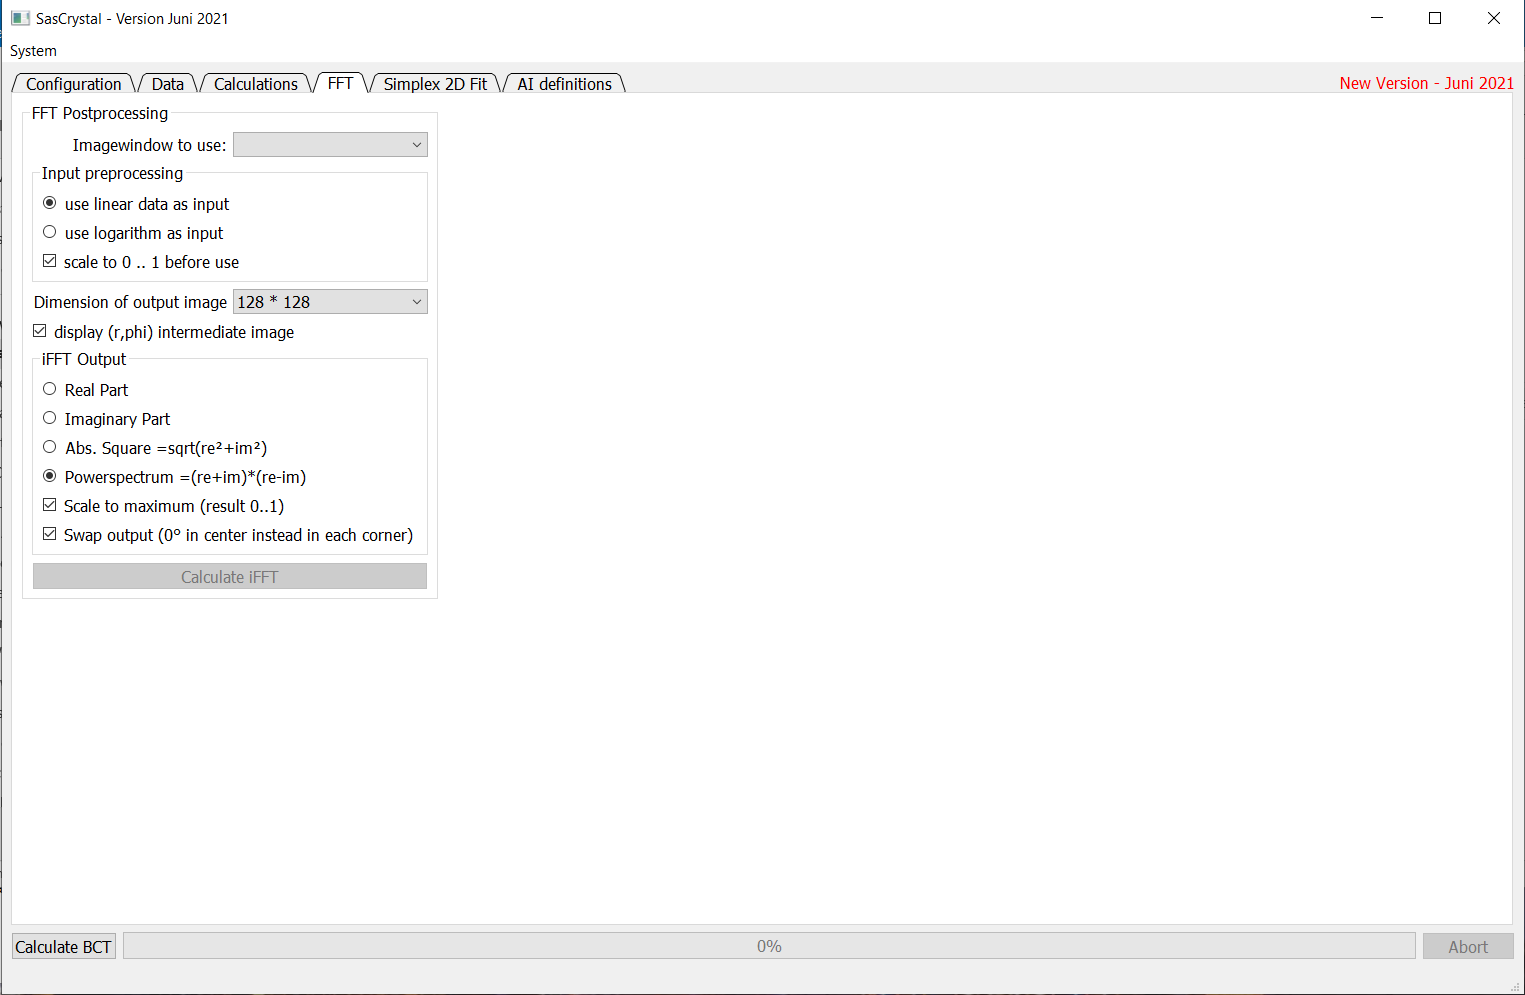
\includegraphics[width=0.96\textwidth]{main-fft-start.png}
 \caption{Fft view after startup.}
 \label{fig:fftstart}
\end{figure}

This postprocessing can be done manually after the calculation of an image or it can be used during image generation for AI (see the AI definition tab). First a (r,phi) Image is calculated from the input image. From this intermediate image the inverse FFT will be calculated. The options in this screen are:
\begin{itemize}\itemsep0pt
\item Imagewindow to use \\
	Here you must select the input image.
\item Input preprocessing \\
	It is possible to use the image data as is (linear) or calculate the logarithm first. You can select the scaling to the range of 0 to 1 or to leave the values unchanged.
\item Dimension of output image \\
	Here you can select the size of the output image (only dimensions of $2^n$ allowed).
\item display (r,phi) intermediate image \\
	If checked, the intermediate image is displayed.
\item iFFT Output \\
	The output image data can be selected and scaled. This is useful for the AI system. The output can be swapped so that the zero is in the center and not at the corners as usual.
\item Calculate iFFT \\
	This button starts the calulation.
\end{itemize}


\subsection{Simplex 2D Fit tab}

To optimize the parameters a {\it Downhill Simplex 2d Fit} algorithm is implemented. It can be started manually in this tab and can work in an automatic mode (described later).

The top line shows the current used calculation method. This can only be changed in the calculation tab.

The left list contains all possible fitable parameters. They are shown with a bold label in the calculation tab. This can be configured with a special config file (see Appendix). For each parameter in this list you can:
\begin{itemize}\itemsep0pt
\item select if this parameter is used for the fit algorithm
\item set the min and max values as the fit limits
\item set the start value for the fit
\item view the result of the last fit run (last column)
\end{itemize}

The list at the right is filled during the fit process if the update flag in the configuration tab is checked. All messages are allways written in a temporary file which might be saved for future use with the button below the list.

\begin{figure}[H]
 \centering
 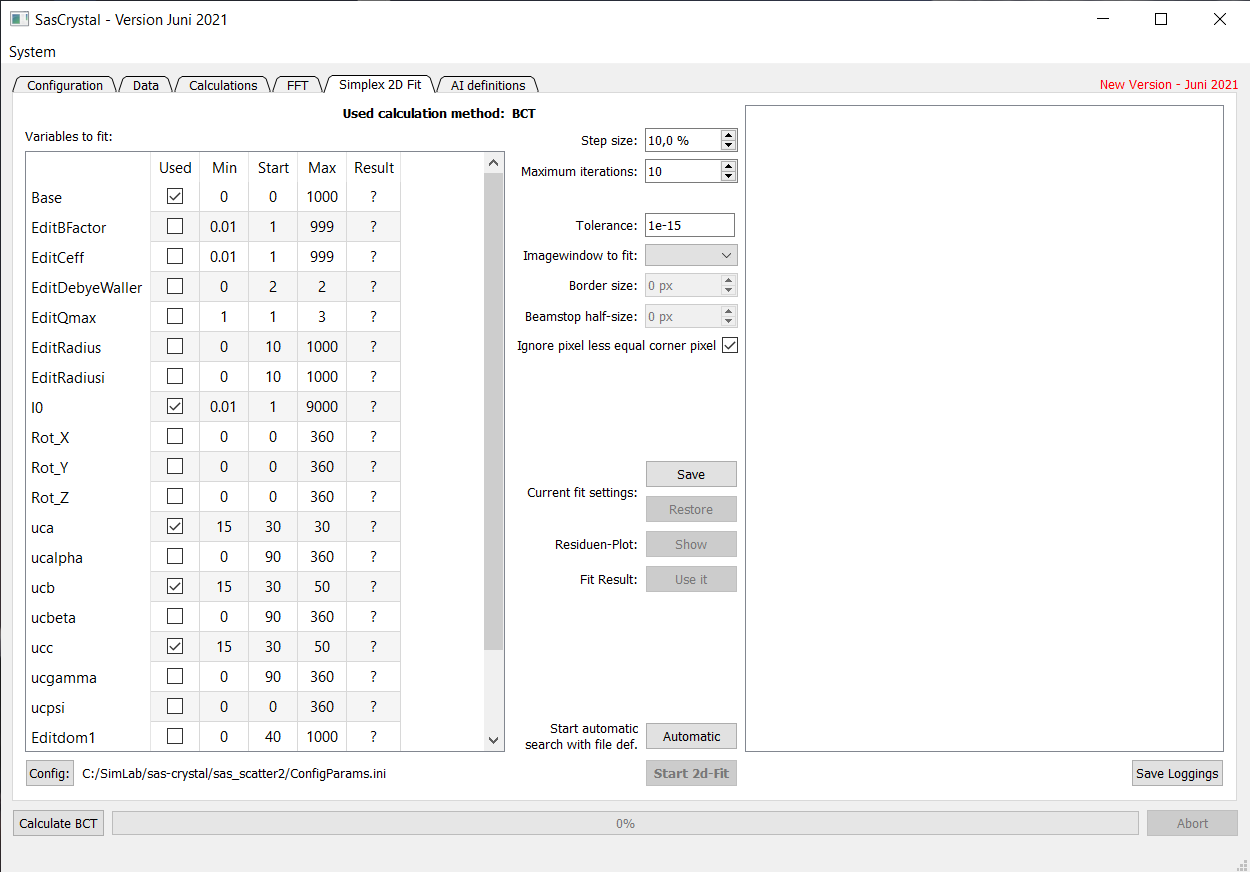
\includegraphics[width=0.96\textwidth]{main-fit-start.png}
 \caption{2D Fit view after startup.}
 \label{fig:fitstart}
\end{figure}

The options in the middle are:
\begin{itemize}\itemsep0pt
\item {\it Step size}: is used to calculate the next values during the fit.
\item {\it Maximum iterations}: is the limit of the fit iterations if the tolerance is not reached.
\item {\it Tolerance}: is the maximum limit of the sum of squared errors.
\item {\it Imagewindow to fit}: is to select which image to be fitted.
\item {\it Border size}: is the number of pixel to be ignored during the fit at each border.
\item {\it Beamstop half size}: is the number of pixel to be ignored around the beam stop.
\item {\it Ignore pixel less equal corner pixel}: if checked, the pixel values above are disabled and all pixel less or equal the corner (first data value) are ignored during the fit. This is often usefull for KWS images.
\item {\it Current fit settings}: the current values in the left list can be saved and reloaded. This is only stored in one memory location, so only one set of values can be saved. The next save overwrites the one before.
\item {\it Residuen Plot}\footnote{This feature is experimental}: this shows a new image with the differences between the original image and the last fit. The negative values are in greyscale and the positive values are in glowing or temperature color tables.
\item {\it Fit result}: sets the current result values as new start values in the calculation tab and in the current settings. After this simply click the Calculate button in the lower left corner and get an image with the fit result.
\item {\it Start automatic}: here you can select a file and some optione (see below) to start the automatic fit process. The file format is described later.
\item {\it Start 2d-Fit}: button starts one fit run with the current settings and displays the result values in the list. No image window will be generated.
\end{itemize}

\begin{wrapfigure}{r}{0.51\textwidth}
  \begin{center}
    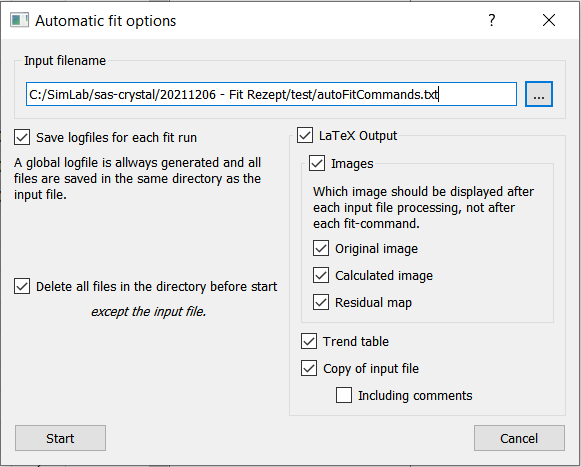
\includegraphics[width=0.5\textwidth]{auto-fit-options.png}
  \end{center}
 %\caption{Visible main menu.}
 %\label{fig:mainmenu}
\end{wrapfigure}
In this automatic fit configuration dialog you can select the input file for the automatic fit and set some ouptions for the generated output. All informations are saved if the start button is clicked. This will start the automatic fit operation.

The most detailed option part is for the \LaTeX\  output file generated. Even if the images are not included in the file, the image files are generated. The Trend table contains all used parameters with all values after each fit run. The input commands can be included in the \LaTeX\  output. It is possible that some characters in the commentlines of the input file can confuse the \LaTeX\ converter, so you can exclude the comments for the output file.

During the fit operations all informations can be saved in special files if the {\it Save logfiles} is checked. One global logfile is generated if the command is included in the command file. The {\it Delete all files} checkbox can be used to delete all files except the input file before the fit run starts.


\clearpage
\subsection{AI definitions tab}

In this tab you can define how a sequence of images will be generated as a training set for a tensorflow neural network with the goal to identify some informations in real measurement data.

\begin{figure}[H]
 \centering
 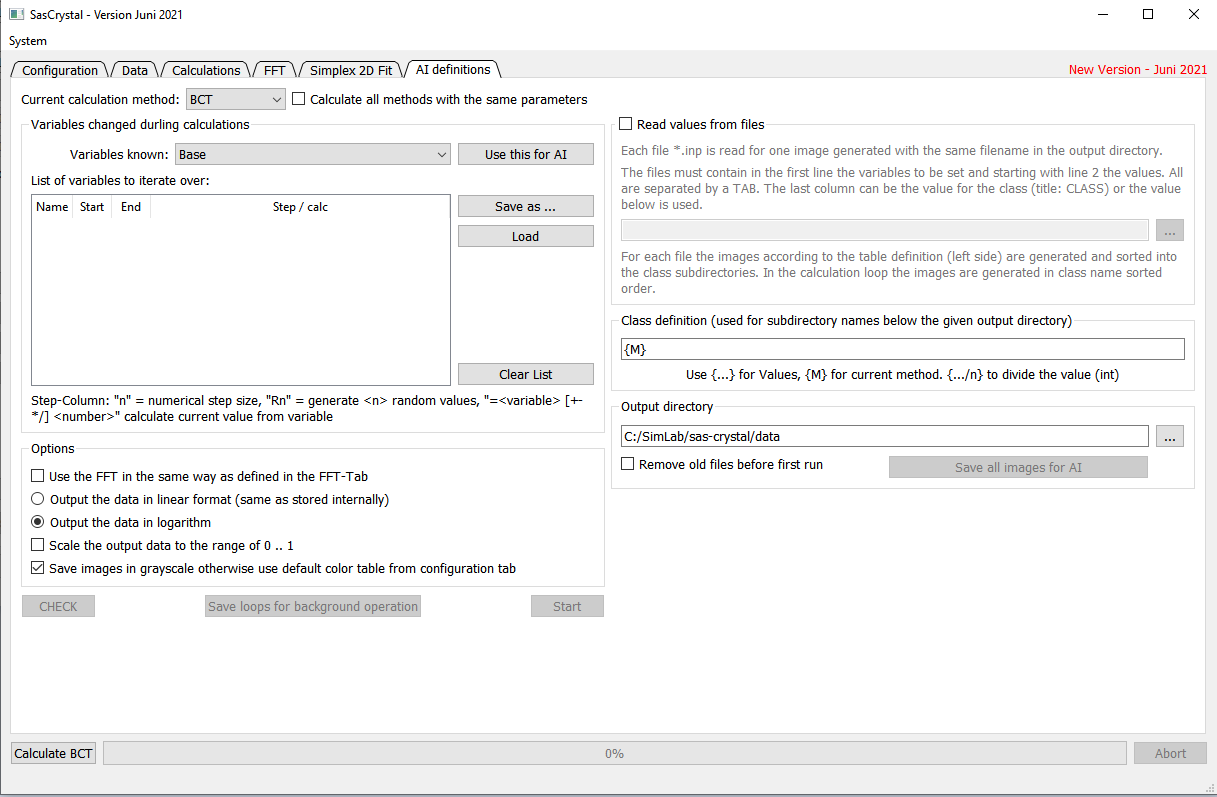
\includegraphics[width=0.96\textwidth]{main-aidef-start.png}
 \caption{AI definition view after startup.}
 \label{fig:aistart}
\end{figure}

The usage might sound a bit complicated. Here I'll describe the input fields, the basic usage is described in a later chapter.
\begin{itemize}\itemsep0pt
\item[-] Left part from top to bottom:
\item Use only one method selected here or use all known methods for the image generation.
\item The variable section shows all parameters to be modified during the generation. The exact usage is described in a later chapter.
\item In the option section you can enable the FFT postprocessing and modify the image output formats.
\item Button {\it CHECK} will check the processing loops and gives an information about how many images and classes will be generated.
\item Button {\it Save loops for background operation} will save the processing informations into a special file which can be read in with the console version of this program to run the calculations without a GUI in the background.
\item Button {\it Start} will start the processing directly: the special file will be generated and the background process is started. From now on you have no control over the background process. So it might be a good idea to start this process from a terminal to get informations about the running process and have control to stop it.
\item[-] Right part from top to bottom:
\item The {\it Read values from files} option can be used to read a list of files (e.g. with different orientation vectors) and for each file the processing defined on the left side is done.
\item The {\it Class definition} is used as the subdirectory name and as a result information for the tensowflow neural network.
\item The {\it Output directory} will be populated with all generated files. it might be a good idea to remove the old imagefiles before processing starts. If you want to have more files because some parameters are randomly generated, then you can leave the old files.
\item With {\it Save all images for AI} will save all open image windows in the directory ``files/'' under the output directory in the same format as the other images will be generated. This is usefull for testing the neural network.
\end{itemize}


\subsection{Image windows}

\begin{wrapfigure}{l}{0.36\textwidth}
  \begin{center}
    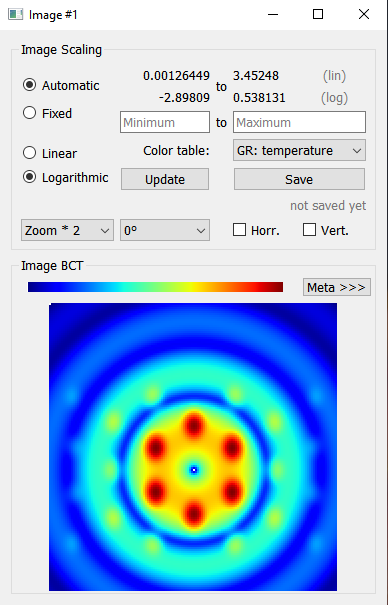
\includegraphics[width=0.35\textwidth]{img-bct.png}
  \end{center}
 \caption{Example image}
% \label{fig:img1}
\end{wrapfigure}
Each calculated image or loaded dataset is displayed in a single window with some visual manipulation functions.

Select the scaling method: {\it Automatic} searches the minimal and maximal value and divide this range by the number of colors in the color table. {\it Fixed} uses the values from the input fields. To make it easier to set the same scaling in different windows, the current min/max values are displayed for the linear mode (e.g. real data values) and for the logarithmic mode (the log of the min/max data values if they are not zero or negative). Then you can select the color table scaling: {\it Linear} or {\it Logarithmic}.

You can select one of four color tables: greyscale, glowing colors, temperature like and earth colors. For the information which color is the min and which is the max, the colorbar is displayed just above the image.

You can set the zoom factor (no zoom, *2, *4, /2, /4), the rotation of the display and the horizontal or vertical mirroring. None of the manipulations will change the internal dataset, it affects only the visible representation.

After each change of the color table, scaling, rotation or mirroring, you have to click on the update button to update the image. Only the zoom factor generates directly a new image.

The save button saves the image in three formats: as an image (*.png), importable into Excel (*.csv) and in binary format (*.dat). The metadata is stored in a simple textfile (*.txt). After saving the path and filename is displayed just below the save button.

The Meta button will show the table of all stored metadata informations on the right side of the window (see figure \ref{fig:imagemeta}). For calculated images, the metadata contains all parameters. For loaded datasets the metadata contains some of the provided header informations. Below this table a small histogram of the data is displayed. This histogram is calculated from the image, not from the real data. The vertical scaling is calculated from the second highest count value divided by the used 60 pixel.
\begin{figure}[H]
 \centering
 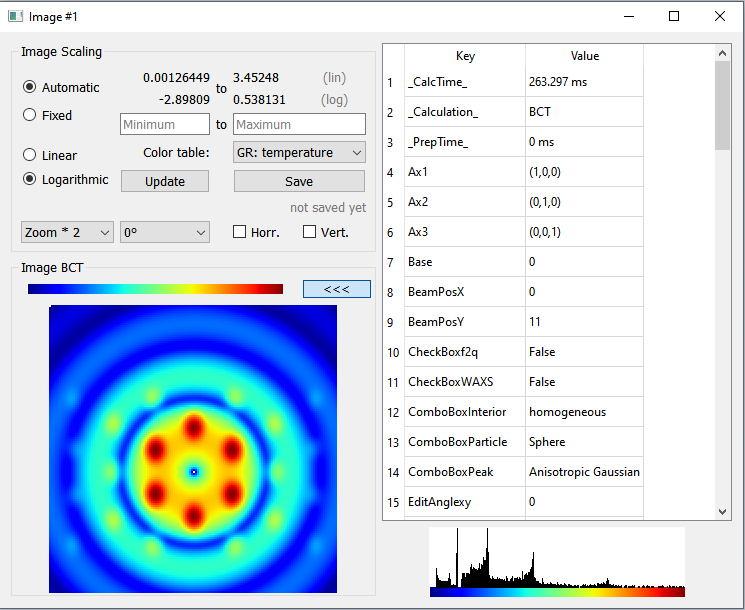
\includegraphics[width=0.67\textwidth]{img-bct-meta.png}
 \caption{Example image with meta data table}
 \label{fig:imagemeta}
\end{figure}


\subsection{Time test dialog}

\begin{wrapfigure}{r}{0.34\textwidth}
  \begin{center}
    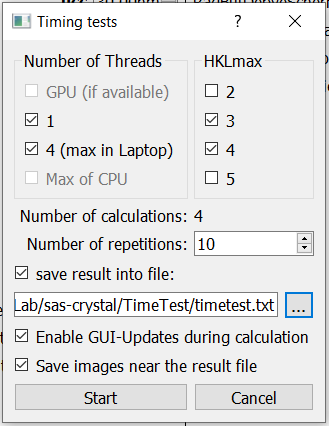
\includegraphics[width=0.3\textwidth]{timing_test.png}
  \end{center}
 \caption{Timinig test definition}
% \label{fig:timetest}
\end{wrapfigure}

This function allows the user to make a simple test of the performance of the current used system.

In the shown dialog the number of used threads are selectable, 1 thread is the slowest, 4 threads are the maximum on my development system (used for comparison), the maximum number of threads are determined by the program. The GPU can be enabled too. If not more than 4 threads possible or if no GPU found, then the apropriate checkboxes are disabled. The value of HKLmax can be set to different values, higher values increases the calculation time.

The program calculates an image with the current parameter settings for each of the combination thread/HKLmax. The images are only saved if the apropriate checkbox is checked. The saved image files have the naming syntax: {\it timetest-t={\bf 1}-hkl={\bf 3}.png}.

This calculations are repeated the given number of repetitions and then the minimal, maximal and mean time are saved to the given result file. During the calculations the current step is shown in the status bar.

The enabling of the GUI updates (progress bar) might increase the calculation time if you are working over the network.

The result file is written to be inserted into a \LaTeX\  {\it longtable} for documentation, the first line will contain the filename of the loaded parameter set. This example calculates a BCT image with the default parameters on my development laptop, the (Prep) means the preparation time used before the image calculation starts.
\begin{lstlisting}[frame=single, xleftmargin=1cm, xrightmargin=1cm]
% Loaded parameter: ?
 & Threads & HKLmax & Min/ Mean/ Max (Prep) in ms
 & 1 & 3 & 587/ 595/ 605 (0)
 & 4 & 3 & 244/ 251/ 263 (0)
 & 1 & 4 & 1191/ 1198/ 1210 (0)
 & 4 & 4 & 479/ 487/ 509 (0)
\end{lstlisting}



%------------------------

\section{Usage and hints}

In these chapters I'll write some informations for the usage of the program.

\subsection{Normal image calculation}

The normal work is very easy: select the method, set the parameters to values you want and press the Calculate button. The bar right of the button shows the progress, it can be very fast. After the calculation the image will be displayed in a new window. Then you can change some parameters and recalculate the image.

\subsection{Working with measurement datasets}

First go to the data tab, then click on the {\it open measurement file} button. You can open different file types (selected by the file extension):
\begin{itemize}\itemsep0pt
\item TIFF-Images (*.tif *.tiff), multiple images are not recognized in the current version
\item KWS-Data (*.dat *.data)
\item ESRF/Klora images (*.edf), might be very large
\item HDF5 Files (*.h5 *.hdf *.hdf5 *.nxs), if more than one image is found, a selection dialog will ask the user which image(s) should be loaded and displayed. If used in the automatic fit, only the first selected image will be used. {\it The meta data usage is under development.}
\end{itemize}
Each data file will be opened in a new window. And the internal flag is set so that the next calculated image will be opened in an other new window. The main goal is to use the measurement data for the 2D Fit.
\begin{figure}[H]
 \centering
 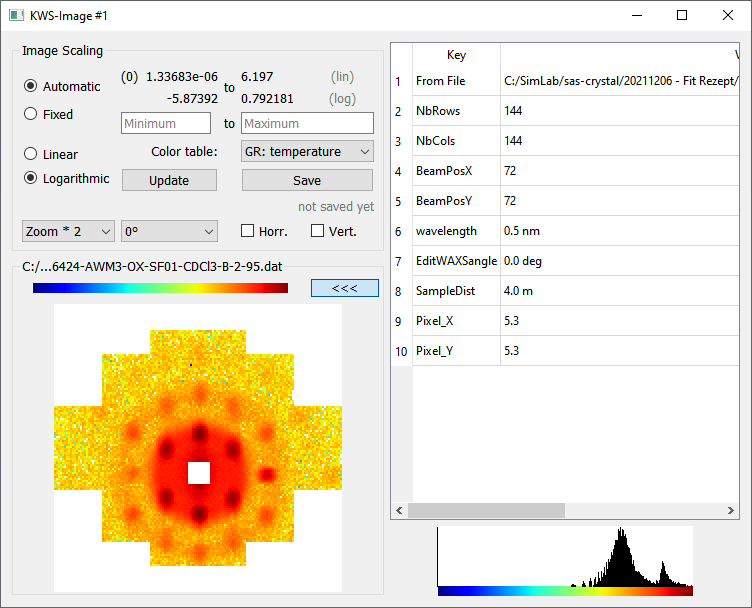
\includegraphics[width=0.67\textwidth]{img-kwsdata-meta.png}
 \caption{Example KWS image with meta data table}
\end{figure}

\subsection{Working with the Simplex 2D Fit}

The implemented Downhill Simplex Algorithm can be used to calculate the parameters to generate an image fitted to the given dataset.

\subsubsection{Manual mode}

The manual fit mode is used to get an idea of some fit parameters. And you can obtain some fit steps to put them later into an automated procedure.

At every fit step you have to think about the variables (which you want to be modified, what is the starting value and what are the limits). Then press the {\it Start 2d-Fit} button. The progress of the fit will be documented in the list box on the right side. At the end the Result column of the variable table will be filled. For the next fit run press the button {\it Fit Result Use it} to copy the result values as the new start values and press the start button again.

If you want to see the result image click on the calculate button (lower left) to get a new or update the last image window. Be sure to klick on the button {\it Fit Result Use it} before calculation.

\subsubsection{Automatic mode}

If you use the manual fit mode, each fit step will be written in the text field in the configuration tab in the syntax to be used for the automatic mode. These steps can be copied into a file to be used as an input for this mode.

The possible commands for this automatic mode input file are:
\begin{itemize}\itemsep0pt
\item {\bf \#} the rest of this line is a comment and will be ignored
\item[] {\it The following commands are only interpreted during the first scan of the file. More scans are done if more than one input file is included.}
\item {\bf GlobLog:} {\it filename} \\
	The given filename is used for the global logfile. If \LaTeX\  output is enabled, the path is used for this output file, the name is fixed to \path{latex-output.tex}.
\item {\bf Param:} {\it filepath} \\
	The parameter input file to be used during the fit.
\item {\bf DirMask:} {\it *.dat} \\
	Filemask used for the DirUp / DirDown commands.
\item {\bf DirUp:} {\it dir} \\
	Directory to be scanned in alphanumeric ascending order.
\item {\bf DirDown:} {\it dir} \\
	Directory to be scanned in alphanumeric descending order.
\item {\bf File:} {\it filepath} \\
	Single file to be used (multiple occurances possible).
\item {\bf Limits:} {\it $<$Parametername$>$; $<$Min$>$; $<$Max$>$} \\
	Set the limits used during the fit for the given parameter (multiple occurances possible).
\item[] {\it The following commands are interpreted at every file scan.}
\item {\bf Info:} {\it informational text} \\
	This text will be shown in the GUI, more than 20 chars can disturb the GUI layout.
\item {\bf Use:} {\it $<$Param1$>$, $<$Param2$>$, ... } \\
	List of parameternames used during the next fit step.
\item {\bf Fit:} {\it Stp=3.0; Iter=20; Tol=0.0010; Diff$<$5} \\
	Perform one fit operation. The values of Stp (Step size), Iter (Maximum iterations), Tol (Tolerance) are the same as in the GUI used for this fit run. After each fit run the percentual change of each parameter is summed up and if this sum is less than the Diff value the fit step is finished. If not, this fit run is repeated up to 20 times to avoid endless loops.
\end{itemize}


\clearpage
\subsection{Generate AI files}

I've played around with some neural networks to find some parameters automatically. For this I used a docker image with a preinstalled tensorflow system. The goal was to train this network with as many images as possible to get a good result.

\subsubsection{Example to use the AI files}



%------------------------
\clearpage
\section{Console version}

To perform the calculation work in a batch job, the console version of the program was written. It was only a wrapper around the same calculation routines as the GUI version. It has no GUI but a lot of calling arguments to configure the calculations. The call is: \\
\centerline{{\bf sas\_scatter2Cons} {\it options and parameters}}

\begin{longtable}{|L{1cm}|L{2cm}|C{2cm}|L{12cm}|}
\caption{Possible options for sas\_scatter2Cons} \\
\hline\rowcolor{rowcolor}{\bf Short} & {\bf Long} & {\bf Parameter} & {\bf Description} \\
\endfirsthead
\hline\rowcolor{rowcolor}{\bf Short} & {\bf Long} & {\bf Parameter} & {\bf Description} \\
\endhead
\hline
-h & -{}-help & & Displays help on commandline options. \\ \hline
 & -{}-help-all & & Displays help including Qt specific options. \\ \hline
-v & -{}-version & & Displays version information. \\ \hline
-p & -{}-paramfile & {\it paramfile} & Filepath loaded as the parameter set for all calculations (*.ini). \\ \hline
-c & -{}-seqfile & {\it aifile} & Filepath loaded as the AI definition sequence (*.sas\_airun). \\ \hline
-i & -{}-img & {\it imgfile} & Filepath and name to save the image (*.png). Or the image to load for automatic fit (*.dat). \\ \hline
-t & -{}-threads & {\it threads} & Number of threads used (default=max cores), set to {\bf 0} to use GPU if available. \\ \hline
-l & -{}-logfile & {\it logfile} & Filepath and name of the logfile for informations of the process (*.log). \\ \hline
 & -{}-csv & {\it csvfile} & Filepath and name of the csvfile for some statistic outputs during 2D-Fit (*.csv). \\ \hline
-f & -{}-autofit & {\it autofit} & Filepath and name for the automatic fit routine (*.txt). If this is given, the AI-File is ignored and the imagefile is an input dataset. \\ \hline
-o & -{}-output & {\it output} & Filepath and name of the single output image of the automatic fit routine or the path to save the  multifile outputs. \\ \hline
-m & -{}-method & {\it method} & Method to be used for single image calculation and 2D-Fit. \\ \hline
 & -{}-nofft & & If set, the FFT calculation during AI generation is skipped. \\ \hline
 & -{}-noconsole & & If set, no output is printed to the console during auto fit (except statistic info). \\ \hline
 & -{}-swap & {\it [HV]} & Set the image swapping and can contain the characters 'H' and/or 'V'. \\ \hline
 & -{}-rotate & {\it [0123]} & Set the image ratoation to 0(=0°), 1(=90°), 2(=180°), 3(=270°). \\ \hline
 & -{}-zoom & {\it [124]} & Set the image zoom factor to 1, 2, 4. \\ \hline
 & -{}-color & {\it color} & Set the used colortable to one of: grey, glow, earth, temp. \\ \hline
\end{longtable}


%------------------------

\clearpage
\appendix

\section{Configuration files}


\section{Content of the git}

If you get access to my git ({\it https://iffgit.fz-juelich.de/wagener/sas-crystal}), you get a lot of directories with all tests, helper programs and development steps. Here I write some informations to each directory\footnote{Some names are in german and some text files too, this is historical.} and some files found in the git:

\begin{longtable}{|L{7.3cm}|L{10.1cm}|}
\hline\rowcolor{rowcolor}{\bf Directory} & {\bf Description} \\
\endfirsthead
\hline\rowcolor{rowcolor}{\bf Directory} & {\bf Description} \\
\endhead
\hline
\path{20200526 - unit cell rotations/} & Informations about unit cell rotations. \\ \hline
\path{20200724 - fit 2d/} & First steps towards the fit algorithm. \\ \hline
\path{20200818 - Read KWS Images/} & First reading of KWS data files. \\ \hline
\path{20200826 - FCC und BCT/} & Differences between FCC and BCT calculations. \\ \hline
\path{20210322 - Radiant und FFT/} & Discussions about the radial average images and the FFT. \\ \hline
\path{20210601 - HDF5/} & First steps to read HDF5 data files. \\ \hline
\path{20210601 - neuer Algorithmus R-PHI/} & Updates of the radial average algorithm. \\ \hline
\path{20210616 - Neue Routinen/} & New routines of the basic pascal program. \\ \hline
\path{20211105 - BCT neu/} & Tests with the new routines. \\ \hline
\path{20211206 - Fit Rezept/} & Tests for the multi-input-file function of the fit algorithm. \\ \hline
\path{20211206 - Fit Rezept/AutoFit/} & Some tests for the automatic fit routines. \\ \hline
\path{20220303-AI/} & Current steps for the new AI approach. \\ \hline
\path{dl_report/} & Helper program to analyze the output files from the Tensorflow run. \\ \hline
\path{docker-tests/} & Docker scripts for the experiments with Tensorflow. \\ \hline
\path{docker-tests/cedric/} & Helper script to generate 3 random vectors standing perpendicular to each other. This is used for the AI generation. \\ \hline
\path{doku/} & First documentations and default save path for the images. \\ \hline
\path{hdf_explorer_qt-master/} & Helper program found in a git repo to explore HDF5 files. \\ \hline
\path{pas2cpp/} & Helper program to convert Pascal code to C++ code. \\ \hline
\path{sas/} & First GUI program without GPU usage. \\ \hline
\path{sas_imageing/} & Helper program (experimental) to erode or dilate an image for the AI algorithm. \\ \hline
\path{sas_report/} & Helper program to generate a report from some logfiles written during 2D fit. \\ \hline
\path{sas_scatter/} & Former version of the GUI / console program before restructuring the algorithms. \\ \hline
\path{sas_scatter2-doc/} & Source of this documentation. \\ \hline
\path{sas_scatter2/} & Software currently used and developed. \\ \hline
%
\path{.gitignore} & List of files / directories ignored by the git. \\ \hline
\path{HDF5 Notizen - H5Einit.h} & After first cmake run of the HDF5 library, the file {\it H5Einit.h} has unexpected line breaks. This is a copy of the edited file. \\ \hline
\path{HDF5 Notizen.txt} & Notes and descriptions to install the HDF5 library. \\ \hline
\path{History.txt} & Description of the first few weeks of development. \\ \hline
\path{*.sas_ai} & Saved files for the AI definitions. \\ \hline
\path{*.ini} & Saved files for all parameters. \\ \hline
\path{README.md} & Readme for the git web interface. \\ \hline
\path{Scatter_pascal.docx} & Some informations from the scatter program with explanations from Prof. Förster. \\ \hline
\path{Upq.pas} & Older source of the pascal program (external functions). The actual versions are in \path{20210616 - Neue Routinen/}. \\ \hline
\path{Vergleich.docx} & Comparison of \path{Scatter_pascal.docx} and \path{crystal3d1.pas}. \\ \hline
\path{crystal3d1-n.pas} & Older source of the pascal program (see above). \\ \hline
\path{crystal3d1-old.pas} & Older source of the pascal program (see above). \\ \hline
\path{crystal3d1.pas} & Older source of the pascal program (see above). \\ \hline
\end{longtable}


\section{Used keys in system setings}

The following keys and groups are used to store informations beyond program run. They are stored in
\begin{itemize}\itemsep0pt
\item {\bf Windows registry:} \path{\HKEY_CURRENT_USER\SOFTWARE\JCNS-1-SasCrystal\}{\it MasterKey}\path{\...}
\item {\bf Linux files:} \path{$HOME/.config/JCNS-1-SasCrystal/}{\it MasterKey}\path{.conf}
\end{itemize}

%\begin{longtable}{|L{7.3cm}|L{10.1cm}|}
\begin{longtable}{|l|l|c|l|}
\hline\rowcolor{rowcolor}{\bf Goup} & {\bf Key} & {\bf Default} & {\bf Description} \\
\endfirsthead
\hline\rowcolor{rowcolor}{\bf Goup} & {\bf Key} & {\bf Default} & {\bf Description} \\
\endhead
\hline
%---MainGui---
%    QSettings sets(SETT_APP,SETT_GUI);
\multicolumn{4}{|c|}{Masterkey: {\it GUISettings} }  \\ \hline
 & LastMethod & -1 & \\ \hline
 & ConfigParamFile & & \\ \hline
 & GUIgeometry & & bytearray with geometry informations for the main window \\ \hline
%    // TAB 0 --- Configuration ---
 & ImgAutoPosit & false & ui-togAutoPosit \\ \hline
 & OnlyNewWindow & false & ui-togOnlyNewWindow \\ \hline
 & LimitRuntimeFlag & false & ui-togLimitRuntime \\ \hline
 & LimitRuntimeValue & 60 & ui-inpLimitRuntime \\ \hline
 & DefColTbl & 1 & ui-cbsDefaultColTbl \\ \hline
%    // TAB 2 --- Calculations ----
 & GridPoints & 64 & ui-inpGridPoints \\ \hline
 & Quadrant & 2 & ui-radQ1,2,4 \\ \hline
 & ExpandImg & true & ui-togExpandImage \\ \hline
%    // TAB 3 --- FFT -------------
 & FFTLinInput & true & ui-radFFTLinInput  \\ \hline
 & FFTScaleInput & true & ui-togFFTScaleInput \\ \hline
 & FFTScaleOutput & true & ui-togIFFTscaled \\ \hline
 & FFTSwapOutput & true & ui-togIFFTSwap \\ \hline
 & FFTsize & 2 & ui-cbsFFTsizeMan \\ \hline
 & DispRphi & true & ui-togDispRphi \\ \hline
 & FFToutput & 0 & 0=Real, 1=Imag, 2=Abs, 3=Spec \\ \hline
%    // TAB 4 --- Fit -------------
Fit-Globals & BeamStop & 0 & ui-inpFitBStop \\ \hline
Fit-Globals & Border & 0 & ui-inpFitBorder \\ \hline
Fit-Globals & MaxIter & 10 & ui-inpFitMaxIter \\ \hline
Fit-Globals & StepSize & 1.0 & ui-inpFitStepSize \\ \hline
Fit-Globals & Tolerance & 0.5 & ui-inpFitTolerance \\ \hline
Fit-Globals & Repetitions & 1 & ui-inpFitRepetitions (not used) \\ \hline
Fit-Globals & UseMask & false & ui-togFitUseMask \\ \hline
%            QStringList slVal = sets.value(k,"0:0:0:0").toString().split(":");
%            _fitLimits *fl = new _fitLimits;
%            fl->used = slVal[0].toInt() != 0;
%            fl->min  = slVal[1].toDouble();
%            fl->max  = slVal[2].toDouble();
%            fl->fitType = static_cast<_fitTypes>(slVal[3].toInt());
%            fl->fitvalid = false;  // fitresult not stored!
Fit-* & \multicolumn{3}{l|}{\it For all known calculation methods} \\ \hline
Fit-* & * & 0:0:0:0 & {\it For all fittable parameters} \\ \hline
%    // TAB 5 --- AI --------------
AI & LastSubDir & . & ui-inpSubDir \\ \hline
AI & Grayscale & false & ui-togGrayscale \\ \hline
AI & FileInputEna & false & ui-grpFileInput \\ \hline
AI & FileInputLast & & ui-inpFileName \\ \hline
AI & FileClass & \{M\} & ui-inpFileClass \\ \hline
AI & GenerateIFFT & false & ui-togAIUseFFTOutput \\ \hline
AI & LinOut & true & ui-radAILinOutput \\ \hline
AI & ScaleOut & false & ui-togAIScaleOutput \\ \hline
AI & Cascading & true & ui-radLoopsCascade (not used, allways true) \\ \hline
AI & LastSaveFile & . &  \\ \hline
AI & LastSaveBkgFile & . &  \\ \hline
%---Measurement file---
 & LastImage & dataPath &  \\ \hline
\multicolumn{4}{|c|}{Masterkey: {\it Parameter} }  \\ \hline
%---Parameter file---
 & LastParam & . & \\ \hline
%---Compare data files---
 & CompareF1 & . &  \\
 & CompareF2 & . &  \\ \hline
%---Autofit---
 & LastAutoFit & . & ui-inpInputfile \\ \hline
 & AutoFitRunLogs & true & ui-togRunLogs \\ \hline
 & AutoFitLatexEna & true & ui-grpLatexEnabled \\ \hline
 & AutoFitLatexImages & true & ui-grpImages \\ \hline
 & AutoFitLatexOrgImgStep & true & ui-togOrgImgStep \\ \hline
 & AutoFitLatexCalcImgStep & true & ui-togCalcStep \\ \hline
 & AutoFitLatexResiduenStep & false & ui-togResiStep \\ \hline
 & AutoFitLatexTrend & true & ui-togLatexTrend \\ \hline
 & AutoFitLatexInput & true & ui-togLatexInput \\ \hline
 & AutoFitLatexComment & false & ui-togLatexComments \\ \hline
 & AutoFitDelFiles & false & ui-togDelFiles \\ \hline
 & AutoFitEditor & &  \\ \hline
%    ui->togMinimalOut->setChecked( data.value("AutoFitMinimalOutput",false).toBool() );

\end{longtable}


\end{document}
